\documentclass[border=0.2cm]{standalone}
\usepackage{tikz}
\usetikzlibrary{calc}

\begin{document}
\thispagestyle{empty}
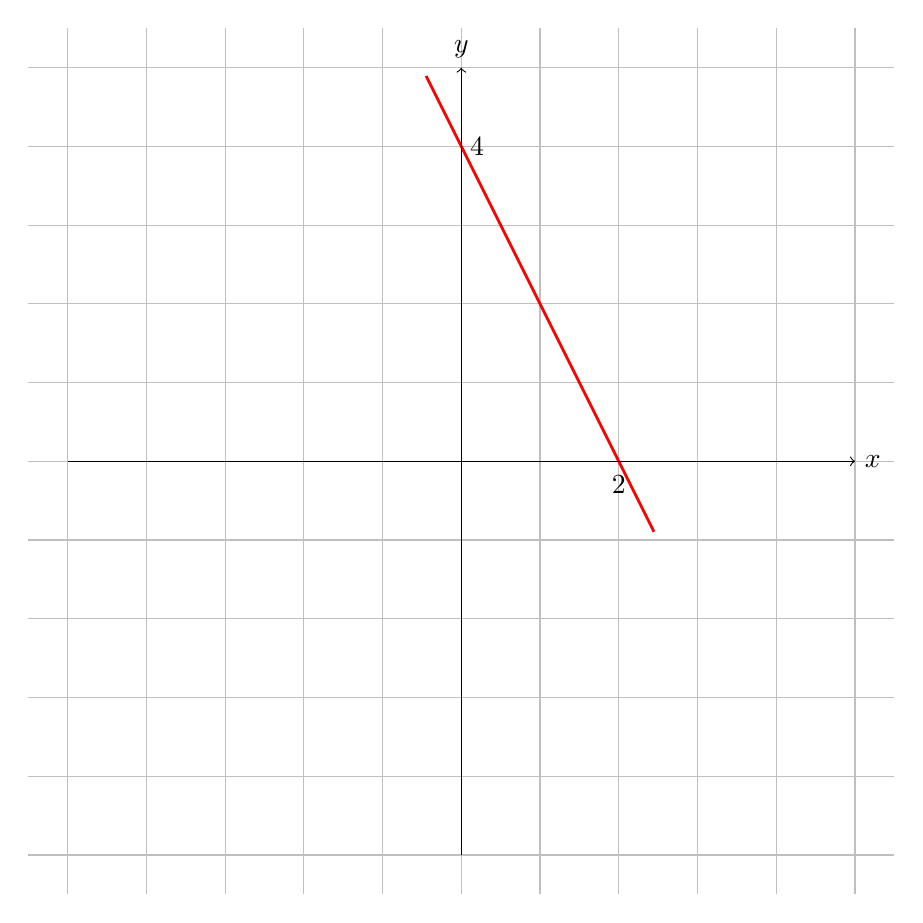
\begin{tikzpicture}[scale=1]
% Desenhar o grid com coordenadas x e y
\draw[step=1,gray!50] (-5.5,-5.5) grid (5.5,5.5);
% Desenhar a reta diagonal com espessura thick e ângulo de 45 graus
\draw[line width=1pt, red] ($(0,4)!-1cm!(2,0)$) -- ($(2,0)!-1cm!(0,4)$);
\node at (.2,4) {4};
\node at (2,-.3) {2};

% Colocar um nó com a letra "b" no ponto (0,2)
%\node at (-0.3,1) {$\bf b$};
%\node[right] at (2,3) { $\bf a > 0$};
% Etiquetas dos eixos x e y
\draw[->] (-5,0) -- (5,0) node[right] {$x$};
\draw[->] (0,-5) -- (0,5) node[above] {$y$};
\end{tikzpicture}


\end{document}
